% !TeX root = ../sustechthesis-example.tex

\chapter[脉冲激光拍频锁定]{脉冲激光拍频锁定}

\textcolor{red}{这部分叙述主要参考文献\cite[]{Islam_Campbell_Choi_Clark_Conover_Debnath_Edwards_Fields_Hayes_Hucul_et_al_2014}}

\section[脉冲激光拍频锁定原理]{脉冲激光拍频锁定原理}
脉冲激光拍频锁定系统原理示意如图\ref{fig:beat_note_stabilization}所示。

\begin{figure}
    \centering
    \caption[脉冲激光拍频锁定系统框图]{脉冲激光拍频锁定系统框图\label{fig:beat_note_stabilization}}
    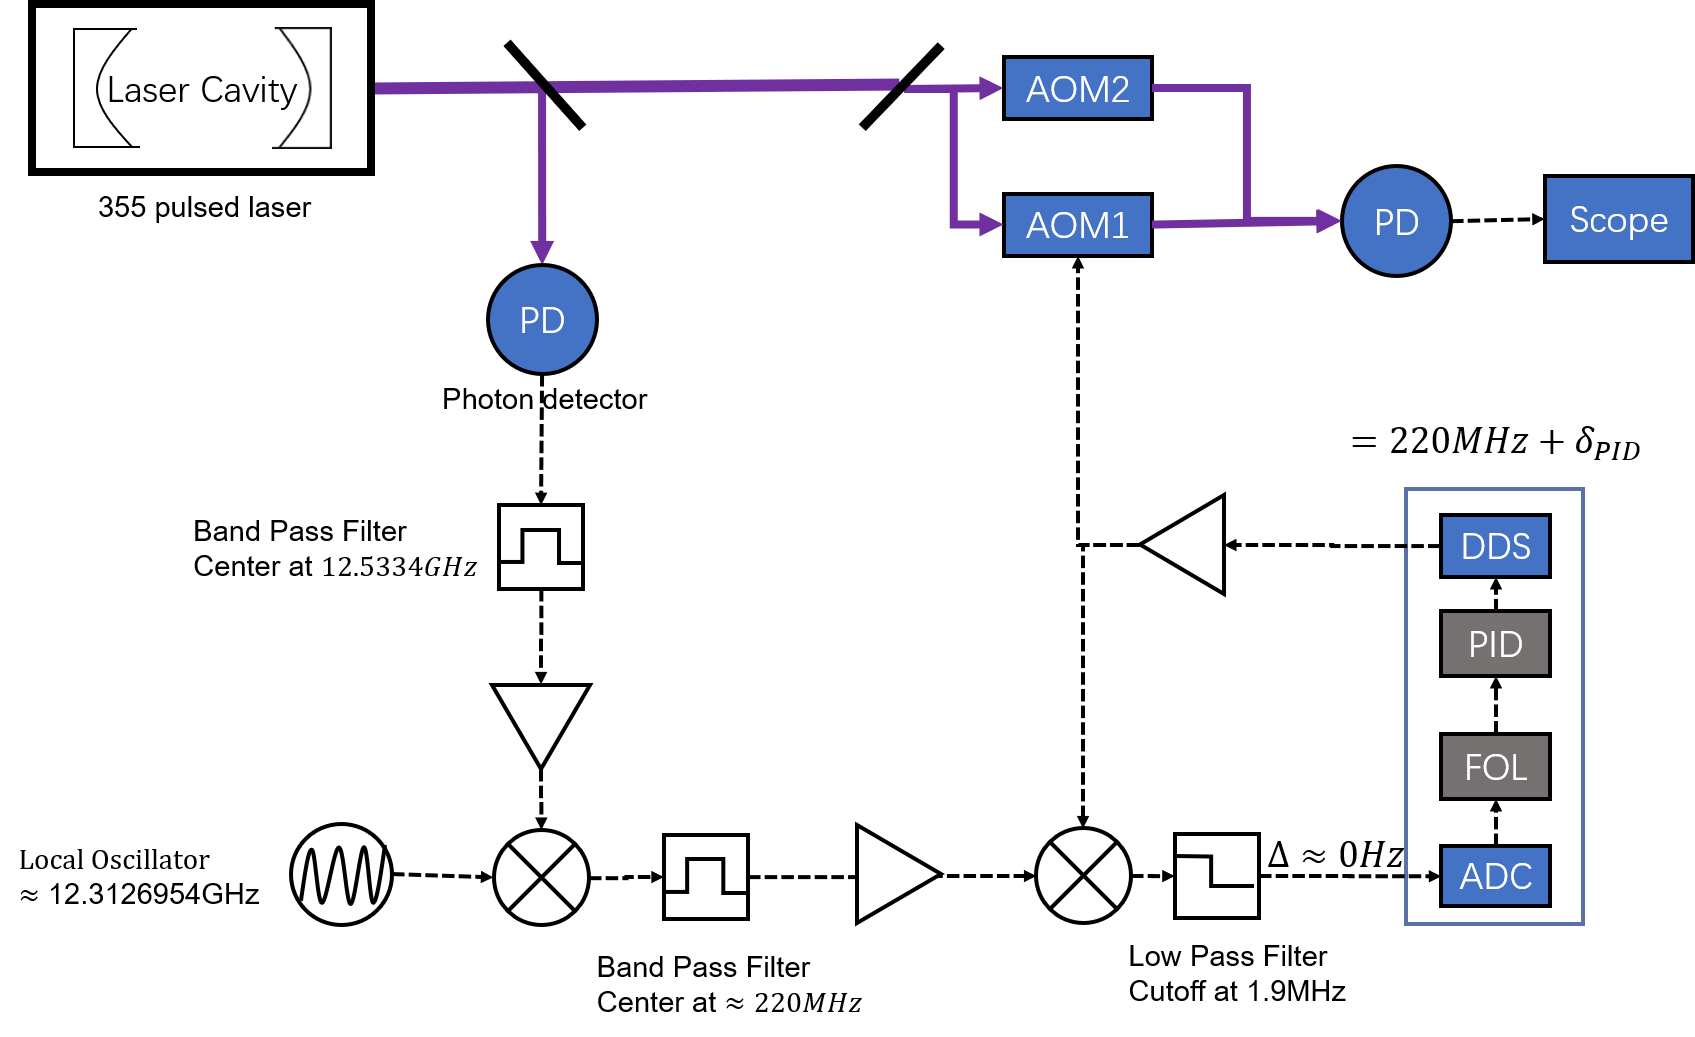
\includegraphics[width=1.0\linewidth]{beat_note_stabilization}
\end{figure}

\section[脉冲激光拍频锁定系统搭建]{脉冲激光拍频锁定系统搭建}
\begin{figure}
    \centering
    \caption[脉冲激光拍频锁定系统图]{脉冲激光拍频锁定系统图\label{fig:beat_note_stabilization_real}}
    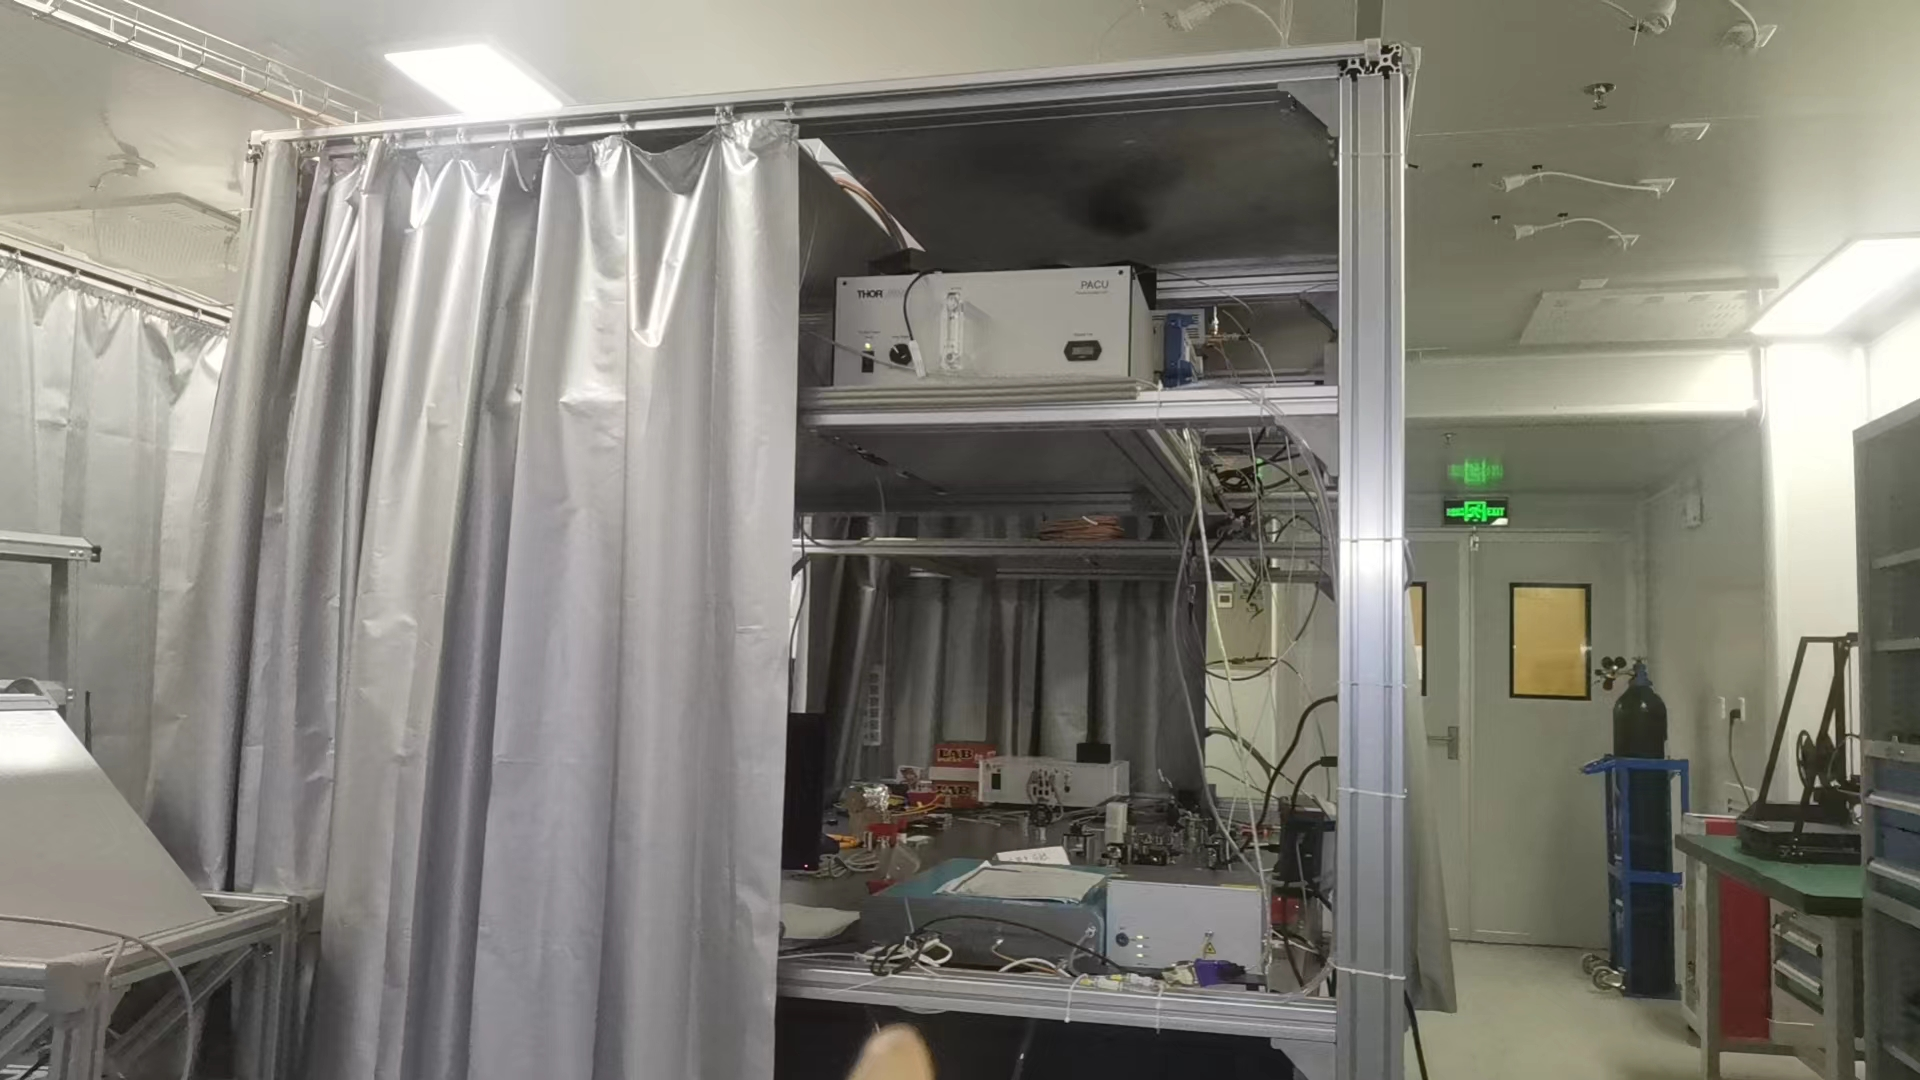
\includegraphics[width=1.0\linewidth]{beat_note_stabilization_real}
\end{figure}
\section[脉冲激光拍频系统锁定结果]{脉冲激光拍频系统锁定结果}

\begin{figure}
    \centering
    \caption[脉冲激光拍频锁定12.39GHz附近稳定边带结果]{脉冲激光拍频锁定12.39GHz附近稳定边带结果\label{fig:beat_note_stabilization_signal}}
    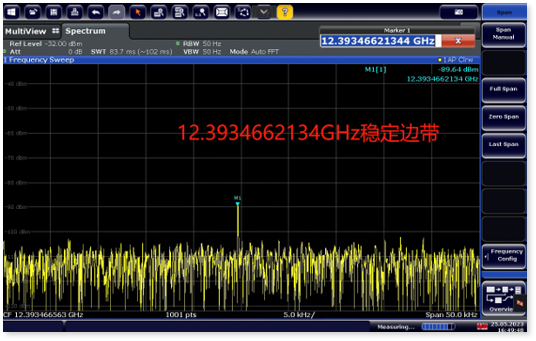
\includegraphics[width=1.0\linewidth]{beat_note_stabilization_signal}
\end{figure}
